\chapter{\IfLanguageName{dutch}{Selecteren frameworks}{Selecting frameworks}}
\label{ch:selecteren-frameworks}

In het vorige hoofdstuk werden de eisen gedefiniëerd waaraan de frameworks binnen deze studie moeten voldoen. In dit hoofdstuk worden alle populaire cross-platform frameworks opgesomd en vervolgens afgetoetst tegen deze eisen. Enkel de frameworks die voldoen aan al deze eisen worden verder in deze studie nog behandeld, de andere frameworks liggen buiten het doel van deze studie. 

Om tot een lijst van de populairste frameworks te komen werd gekeken naar de resultaten van een wereldwijde ondervraging door JetBrains \autocite{Liu2020}. Met 19696 deelnemers aan deze ondervraging is dit een zeer goede weergave van de populariteit van de verschillende frameworks onder ontwikkelaars. In de volgende sectie worden de populairste cross-platform frameworks uit deze ondervraging opgesomd. Vervolgens worden deze frameworks afgetoetst tegen de gestelde eisen. 

\section{Populairste cross-platform frameworks}
\label{sec:poplairsteFrameworks}

In figuur \ref{fig:frameworkPopularity} zijn de resultaten van de ondervraging door JetBrains te zien. Uit deze figuur blijkt dat er enkele zeer populaire frameworks zijn, waarvan React Native en Flutter de populairste zijn. Een interessante opmerking is dat de populariteit van Flutter sterk gestegen is (+9\%) in 2020 in vergelijking met 2019, waar die van React Native hetzelfde gebleven is (42\%). Anderzijds is de populariteit van enkele andere frameworks sterk gedaald: Cordova (-11\%), Ionic (-10\%) en Xamarin (-12\%) zijn een heel pak gebruikers kwijt geraakt. Tot slot zijn helemaal rechts enkele frameworks te zien die in 2019 door geen enkele van de ondervraagden gebruikt werden maar in 2020 wel een bepaald (weliswaar laag) percentage gebruikers weten te overtuigen. Zo duikt bijvoorbeeld Kotlin Multiplatform op in de ondervraging, met 2\% van de ondervraagden die aangeven dit te gebruiken. Ook Kivy en Corona duiken op in de resultaten van de ondervraging in 2020 met elk 1\% van de ondervraagden die aangeeft er gebruik van te maken.

Alle frameworks die aan bod komen in deze ondervraging zullen in de volgende sectie kort besproken worden en vervolgens afgetoetst worden tegen de gestelde eisen (behalve Apache Flex en Dojo, gezien de reeds beperkte populariteit in 2019 en de daling in populariteit in 2020). Het is namelijk niet automatisch zo dat het (op dit moment) populairste framework ook meteen de beste keuze is voor de komende jaren.

Verder wordt ook .NET MAUI besproken in deze studie. Dit is een cross-platform framework dat op 19/5/2020 uitgebracht werd door Microsoft. Omdat delaware een partner is van Microsoft en het team reeds werkt met .NET voor de ontwikkeling van de backend van de applicaties is het zeker een interessant framework om mee te nemen in de vergelijking. Recentere frameworks hebben namelijk het voordeel dat ze enkele tekortkomingen van eerdere frameworks makkelijker kunnen opvangen en kunnen dus zeker ook een goede keuze zijn voor de toekomst.

\begin{figure}
    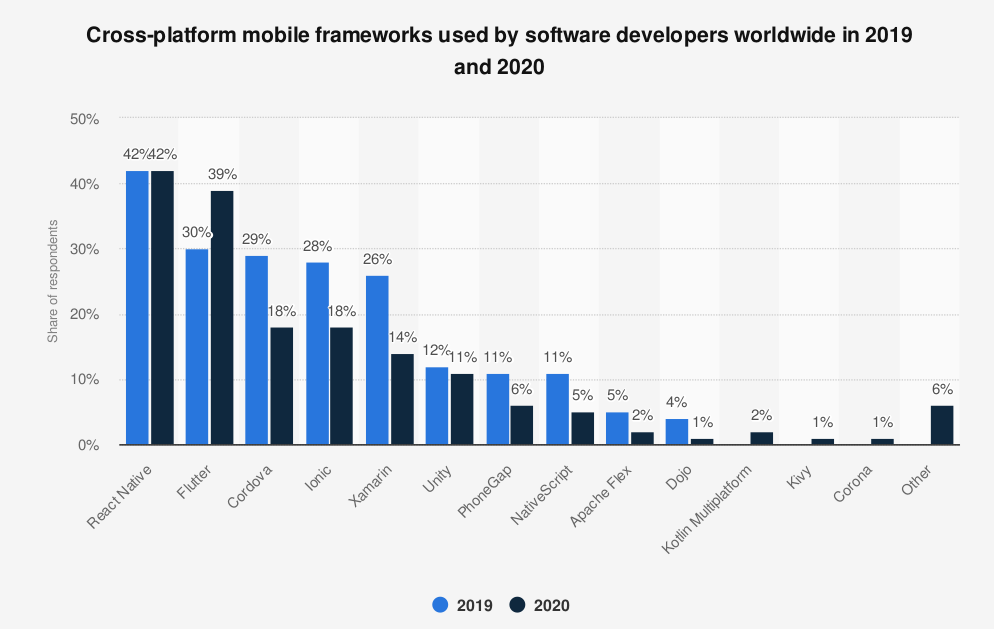
\includegraphics[width=\linewidth]{PopularFrameworksGraph.png}
    \caption{Resultaten van de populariteitsondervraging van cross-platform frameworks door JetBrains}
    \label{fig:frameworkPopularity}
\end{figure}

\section{Achtergrond frameworks}
\label{sec:achtergrondFrameworks}

In deze sectie wordt de achtergrondinformatie van alle frameworks die aan bod komen in de ondervraging van JetBrains kort besproken. Vervolgens worden ze één voor één afgetoetst aan de in hoofdstuk \ref{ch:eisen-framework} gestelde eisen. De frameworks die aan alle eisen voldoen worden vervolgens uitgebreid voorgesteld in hoofdstuk ... 

\subsection{React Native}
\label{subsec:ReactNative}

React Native (2015) is een open source cross-platform framework dat ontwikkeld is en onderhouden wordt door Facebook \autocite. Zoals de naam al doet vermoeden steunt dit framework op React (een Javascript library, ook ontwikkeld door Facebook). React is speciaal ontwikkeld om gebruikersinterfaces te maken, maar waar React zelf zich richt op webbrowsers focust React Native zich op mobiele platformen. Met behulp van React Native kunnen applicaties geschreven worden die er helemaal native uitzien en dit in een taal die reeds heel erg gekend is onder ontwikkelaars \autocite{Eisenman2015}.

\subsection{Flutter}
\label{subsec:Flutter}

Flutter is een software development kit (SDK) ontwikkeld door Google in 2017. Het is een 'UI toolkit' om native gecompileerde apps te maken die er mooi uizien met een enkele broncode \autocite{Google2020}. Net zoals React Native is ook Flutter volledig open source. Het kan rekenen op een grote community en voortdurende verdere ontwikkeling. De laatste stabiele versie van Flutter werd uitgebracht door Google op 6/5/2020. Het is dus een zeer recente update waardoor de SDK kan rekenen op de laatste nieuwe ontwikkelingen op het vlak van cross platform development. Flutter apps worden geschreven in Dart, een object georiënteerde programmeertaal gebaseerd op klassen en ontwikkeld door Google. Het grote voordeel van Dart is dat het gecompileerd kan worden naar Javascript maar ook rechtstreeks naar native code, wat een groot voordeel oplevert op het vlak van prestaties.

\subsection{Cordova}
\label{subsec:Cordova}

Cordova is een framework dat ontwikkeld is door Adobe en bestaat al sinds 2011 (toen nog onder de naam PhoneGap). Het werd in 2013 overgedragen aan Apache om het open source karakter van het framework te kunnen garanderen . Het framework kan gebruikt worden voor het ontwikkelen van cross-platform mobiele applicaties. De talen die gebruikt worden zijn HTML5, CSS3 en Javascript \autocite{Apache2020}. Dit zijn de standaard talen voor de ontwikkeling van webapplicaties, een ontwikkelaar moet dus geen nieuwe taal leren om met Cordova aan de slag te gaan. Applicaties worden uitgevoerd binnen specifieke wrappers per platform en maken gebruik van de native API's om de specifieke hardware componenten van een systeem te gebruiken.

\subsection{Ionic}
\label{subsec:Ionic}

Ionic is een UI toolkit voor het maken van mobiele webapplicaties. Het is ontwikkeld door Ionic zelf en is een open source project. Ionic bestaat uit drie lagen. De basis is Apache Cordova: het is dus een distributie van Cordova en voegt hier extra eigenschappen aan toe. Bovenop Cordova is er een frontend framework geplaats voor het ontwikkelen van de gebruikersinterface. In de eerste versies van Ionic was dit Angular, maar sinds versie 4 is de gebruiker zelf vrij om te kiezen. Er is ondersteuning aanwezig voor Angular, React, Vue.js en web componenten \autocite{Schiemann2019}. Ionic geeft de ontwikkelaar dus zelf de keuze met welk frontend framework gewerkt wordt. De laatste laag tot slot is het Ionic framework zelf: de visuele weergave van het framework en een set van componenten die het mogelijk maken om op een eenvoudige manier de gebruikersinterface te beschrijven.

\subsection{Xamarin}
\label{subsec:Xamarin}

Xamarin is een uitbreiding van het .NET platform van Windows. Het levert een framework dat toegang geeft tot de native eigenschappen van een platform, libraries om de native API's te kunnen gebruiken en een eigen markup taal (XAML) om de gebruikersinterface te beschrijven \autocite{Microsoft2020}. Het grote voordeel van het feit dat Xamarin .NET uitbreid is dat alle mogelijkheden en ondersteuning van .NET ook beschikbaar is voor Xamarin. Ontwikkelaars die reeds gewoon zijn om met .NET te werken kunnen dus onmiddelijk aan de slag met het ontwikkelen van mobiele applicaties met dit framework.

\subsection{Unity}
\label{subsec:Unity}

Unity is een cross-platform framework dat zich richt op het ontwikkelen van games voor mobiele apparaten. Het is uitermate geschikt voor het creëeren van 3D content en complexe graphics. 

\subsection{PhoneGap}
\label{subsec:PhoneGap}

PhoneGap is, net als Ionic, een distributie van Apache Cordova. Het steunt op dezelfde principes maar heeft een eigen gebruikersinterface en extra services. Het is in handen van Adobe (de originele ontwikkelaar van Cordova). Hoewel het in se dus hetzelfde is als Cordova, zijn er bij PhoneGap enkele functionaliteiten extra van Adobe (zoals PhoneGap Build Service, een service die ontwikkelaars toelaat om apps te builden in de cloud).

\subsection{NativeScript} 
\label{subsec:NativeScript}

NativeScript is een open source framework voor het bouwen van mobiele applicaties die native aanvoelen. Net als bij Ionic kan er gebruik gemaakt worden van verschillende frontend frameworks (Angular en Vue.js) of de ontwikkelaar kan aan de slag met JavaScript of TypeScript \autocite{NativeScript2020}. Het grootste voordeel van NativeScript is dat het rechtstreekse toegang geeft tot de native API's. De ontwikkelaar moet dus niet wachten tot iemand een brug geschreven heeft om nieuwe eigenschappen te gebruiken. Van zodra nieuwe eigenschappen beschikbaar zijn van een platform kan de ontwikkelaar deze gebruiken. NativeScript is dus geen wrapper rond een WebView, in tegenstelling tot vele andere cross-platform frameworks \autocite{Anderson2016}.

\subsection{Kotlin Multiplatform}
\label{subsec:Kotlin}

Kotlin is een open source SDK die de ontwikkelaar toelaat om cross-platform applicaties te schrijven en uitgebracht is door JetBrains. Door het feit dat dit een SDK is kan de ontwikkelaar delen van de applicatie in Kotlin schrijven, zonder dat de gehele applicatie opnieuw geschreven hoeft te worden (zoals wel het geval is bij een framework). Verder laat Kotlin Multiplatform ook toe om toch platform specifieke code te schrijven indien er zaken zijn die niet cross-platform opgelost kunnen worden. Door deze mogelijkheid kan de ontwikkelaar ook onmiddelijk inspringen op nieuwe eigenschappen van een platform: van zodra een eigenschap beschikbaar is kan deze ook gebruikt worden in de applicatie \autocite{JetBrains2020}. De mogelijkheid voor het schrijven van cross-platform applicaties met Kotlin is wel nog een experimentele functionaliteit, die beschikbaar is sinds versie 1.3 \autocite{Belov2018}.


\subsection{Kivy}
\label{subsec:Kivy}

Kivy is een open source grafische gebruikersinterface library die het mogelijk maakt om met Python cross-platform mobiele applicaties te schrijven \autocite{Vasilkov2015}. Het stelt de ontwikkelaar in staat om innovatieve gebruikersinterfaces te maken, zoals multi-touch apps. Het is in staat om zware grafische gebruikersinterfaces te tonen en dus ook geschikt voor het ontwikkelen van mobiele games \autocite{Kivy2020}. De eerste release van de library was op 1/2/2011. Het is dus een library die al een tijdje mee gaat en dus geen last meer heeft van kinderziektes.

\subsection{Corona}
\label{subsec:Corona}

Corona is een cross-platform framework dat ideaal is voor het snelle ontwikkelen van mobiele applicaties en games. Het is gebaseerd op Lua, een open source scipting taal. Er zijn vele plugins beschikbaar en er is toegang tot de native API's indien er geen plugin beschikbaar is voor een bepaalde eigenschap. Het framework beschikt over een simulator die de ontwikkelaar toelaat om aanpassingen direct te kunnen zien \autocite{Coronalabs2020}. Een nadeel is wel dat het bedrijf achter Corona niet meer bestaat sinds 1/5/2020. De software gaat verder als een open source project, maar het toekomstige bestaan en updates zijn dus niet langer gegarandeerd \autocite{Shcherban2020}.

\subsection{.NET MAUI}
\label{subsec:.NETMAUI}

.NET MAUI (Multi-platform App UI) is een cross-platform framework dat op 19/5/2020 uitgebracht werd door Microsoft. Op de datum van schrijven van deze studie is dit dus nog een zeer recent framework, dat nog niet veel bekendheid en gebruikers heeft. Het is een verdere evolutie van Xamarin, een ander cross-platform framework van Microsoft. Microsoft heeft als doel om met .NET MAUI een framework aan te bieden dat niet enkel dient om applicaties te schrijven voor smartphones, maar ook voor computers, tablets en andere apparaten waarop applicaties geïnstalleerd kunnen worden. Zoals de naam al doet vermoeden steunt het framework op .NET. Ontwikkelaars die reeds ervaring hebben met dit framework (en C\#, de taal die gebruikt wordt bij .NET) hoeven dus geen nieuwe taal of nieuw framework te leren. De effectieve release van een stabiele versie van het framework is gepland samen met het uitbrengen van .NET 6 in november 2021 \autocite{Hunter2020}. Vanaf deze release is het de bedoeling dat .NET MAUI Xamarin vervangt. Xamarin zal wel nog onderhouden worden, maar alle nieuwe ontwikkelingen zullen in .NET MAUI komen.

\section{Aftoetsen eisen framework}
\label{sec:aftoetsenEisen}

De populairste cross-platform frameworks van de voorbije twee jaar werden besproken in de vorige sectie. In deze sectie worden de verschillende frameworks afgetoetst tegen de gestelde eisen om op deze manier tot een finale lijst van frameworks te komen die in de rest van de studie met elkaar vergeleken zullen worden.

\subsection{Functionele eisen}
\label{subsec:aftoetstenFunctioneleEisen}

De funtionele eisen die gesteld worden aan het framework zijn te vinden in sectie \ref{sec:functioneleEisen}. Al de hiervoor vooropgestelde frameworks voldoen aan alle functionele eisen die gesteld worden aan het framework. Deze worden dus niet afzonderlijk opgesomd. Om tot een verkleinde lijst van frameworks te komen om te kunnen gaan vergelijken moet er dus gekeken worden naar de niet-functionele eisen.

\subsection{Niet-functionele eisen}
\label{subsec:aftoetsenNietFunctioneleEisen}

De niet-fuctionele eisen voor het framework zijn te vinden in sectie \ref{sec:nietFunctioneleEisen}. In tabel \ref{tab:nietFunctioneleEisen} is een overzicht van de resultaten van de verschillende frameworks raadpleegbaar. In de daaropvolgende subsecties wordt uitleg gegeven bij de frameworks die niet voldoen aan de gestelde niet-functionele eisen.

\begin{table}
    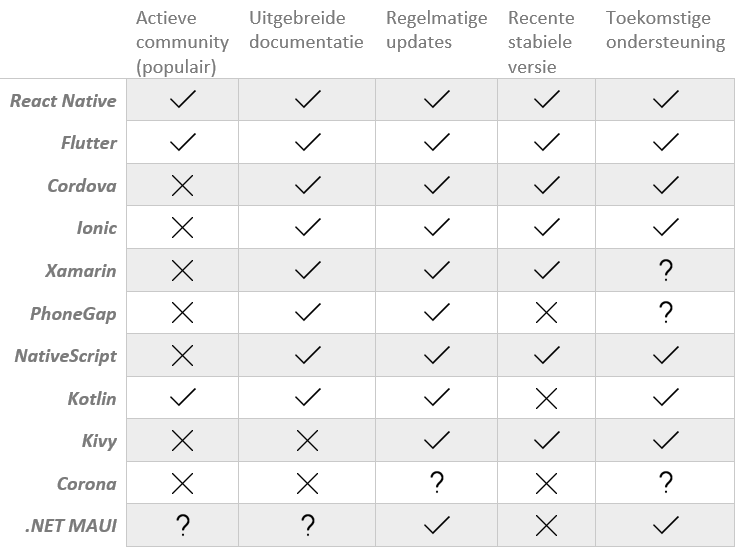
\includegraphics[width=\linewidth]{TabelNietFunctioneleEisen.png}
    \caption{Overzicht aftoetsing niet functionele eisen}
    \label{tab:nietFunctioneleEisen}
\end{table}

\subsubsection{Cordova}
\label{subsubsec:CordovaEisen}

Zoals in tabel \ref{tab:nietFunctioneleEisen} te zien is voldoet Cordova aan alle niet-functionele eisen, behalve aan de populariteitseis. In figuur \ref{fig:frameworkPopularity} is te zien dat de popolariteit van het framework sterk gedaald is. Aangezien het framework  de komende jaren gebruikt zal worden is het ook belangrijk dat het framework populair blijft. Een hoge populariteit geeft namelijk meer opties om te gaan gebruiken (denk aan libraries, oplossingen voor specifieke problemen, ...) en is een goede indicatie of het framework zich kan weren tegen andere frameworks. Cordova verliest vele gebruikers aan andere frameworks, waaruit afgeleid kan worden dat andere frameworks een betere optie zijn om te gebruiken.

\subsubsection{Ionic}
\label{subsubsec:IonicEisen}

Aangezien Ionic een distributie is van Cordova en in figuur \ref{fig:frameworkPopularity} te zien is dat ook de populariteit van dit framework sterk gedaald is kan dezelfde conclusie getrokken worden als bij Cordova.

\subsubsection{Xamarin}
\label{subsubsec:XamarinEisen}

In figuur \ref{fig:frameworkPopularity} is een vraagteken te zien bij de toekomstige ondersteuning van Xamarin. Dit komt doordat Microsoft in mei 2020 een nieuw cross-platform framework heeft uitgebracht (.NET MAUI). Microsoft heeft aangekondigd dat Xamarin wel nog onderhouden zal worden maar dat alle nieuwe eigenschappen in .NET MAUI zullen verschijnen en niet langer in Xamarin. Het nieuwe framework is dus eigenlijk de opvolger van Xamarin, waardoor Xamarin geen goede keuze is om de komende jaren op in te zetten.

\subsubsection{NativeScript}
\label{subsubsec:NativeScriptEisen}

NativeScript is een framework dat net als Cordova en Ionic moet inboeten aan populariteit ten opzichte van andere frameworks. Ook hier kan dus dezelfde conclusie getrokken worden dat dit geen goede keuze is om de komende jaren op in te zetten.

\subsubsection{Kivy}
\label{subsubsec:KivyEisen}

Kivy is een library die al een hele tijd bestaat, en toch weet deze slechts een zeer klein deel van de ontwikkelaars te overtuigen om het te gebruiken. Verder is ook de documentatie eerder beperkt. Het is dus geen goede optie om de komende jaren hier op in te zetten.

\subsubsection{Corona}
\label{subsubsec:CoronaEisen}

Het grootste probleem van Corona is dat het bedrijf achter het framework niet langer bestaat. Er is dus geen gegarandeerde support in de toekomst, er zijn geen recente stabiele versies beschikbaar en het is een framework dat absoluut niet populair is (figuur \ref{fig:frameworkPopularity}). Ook dit framework is dus geen goede optie om de komende jaren op in te zetten.

\section{Finale lijst voor vergelijking}
\label{sec:finaleLijst}

Uit de vorige sectie kan afgeleid worden dat er slechts enkele frameworks zijn die in aanmerking komen om de komende jaren mee aan de slag te gaan. De andere frameworks hebben ook zeker elk hun sterke eigenschappen maar zijn om verschillende redenen (die in sectie \ref{sec:aftoetsenEisen} beschreven staan)) geen goede keuze om de komende jaren applicaties mee te gaan schrijven als bedrijf. De frameworks die hier wel voor in aanmerking komen zullen verder in deze studie tot in het detail besproken worden en nadien onderling vergeleken worden op enkele belangrijke punten. De uiteindelijke frameworks die in deze studie vergeleken zullen worden zijn:

\begin{itemize}
    \item React Native
    \item Flutter
    \item Kotlin Multiplatform
    \item .NET MAUI
\end{itemize}


